\documentclass[sigconf]{acmart}
% Cleaning 
\pagestyle{fancy} % removes running headers
\settopmatter{printacmref=false} % Removes citation information below abstract
\renewcommand\footnotetextcopyrightpermission[1]{} % removes footnote with conference information in first column
\pagestyle{plain} % removes running headers
\fancyhead{}
\settopmatter{printacmref=false, printfolios=false}
% Copyright
\setcopyright{none}
% \setcopyright{acmcopyright}
% \setcopyright{acmlicensed}
% \setcopyright{rightsretained}
% \setcopyright{usgov}
% \setcopyright{usgovmixed}
% \setcopyright{cagov}
% \setcopyright{cagovmixed}
\settopmatter{printacmref=false} % Removes citation information below abstract
\acmDOI{}

\usepackage{booktabs} % For formal tables
\usepackage{url}
\usepackage{algorithm}
\usepackage{tabularx}
\usepackage[noend]{algpseudocode}
\algtext*{EndWhile}% Remove "end while" text
\algtext*{EndIf}% Remove "end if" text
%\usepackage{flexisym}

\setlength{\parskip}{0pt}
\setlength{\parsep}{0pt}
\setlength{\headsep}{0pt}
\setlength{\topskip}{0pt}
\setlength{\topmargin}{0pt}
\setlength{\topsep}{0pt}
\setlength{\partopsep}{0pt}
%\linespread{0.95}
\usepackage{mdwlist}
\usepackage{amsmath}

\begin{document}
\title{Query refinement: type aware approach}
\titlenote{https://github.com/ZahraTaherikhonakdar/Proposed-Solution-Query-refinement-type-aware-approach}
\author{Zahra Taherikhonakdar}
\affiliation{
  \institution{University of Windsor}
%   \streetaddress{P.O. Box 1212}
%   \city{Toronto} 
%   \state{ON} 
%   \country{Canada} 
%   \postcode{43017-6221}
}
\email{taherik@uwindsor.ca}
\author{Aaditya Pradipbhai Parekh}
% \authornotemark[1]
\orcid{0000-0002-6033-6564}
\affiliation{
 \institution{University of Windsor}
%   \city{Fredericton} 
%   \state{NB} 
%   \country{Canada} 
}\email{parekh23@uwindsor.ca}

\begin{abstract}
The goal of this proposed method is to investigate whether considering query types in query refinement (QR) improves the performance of information retrieval (IR) performance. Knowing what refinement methods perform better on what query types could lead search engines to select the best refinement methods based on given query types. In this paper, we define the problem that we will solve and formalize it. The proposed method is also presented. 
\end{abstract}

\keywords{Query Refinement, Query Types, Information retrieval}
\maketitle


\section{Problem Definition}
Considering the query types, the goal is to specify the query refinement methods that improve the information retrieval performance. Here, we provide a formal definition of the problem, after which we propose our approach in detail in the next section. We define the input as a set of queries as $\mathcal{Q}={q_1, q_2,..,q_n}$. Each ${q_n} \in \mathcal{Q}$ is categorized into $n$ query types as $\mathcal{T}={t_1, t_2,...,t_n}$, $\forall{q_n}\in\mathcal{Q},\exists{t_n}\in\mathbb{T}: {q_n}\in{t_n}$, ${t_n}\subset{\mathcal{Q}}$. Each query refinement methods $\mathcal{M}={m_1, m_2, ..,m_n}$ is performed on each input ${q_n}\in\mathcal{Q}$. The refined query ${q^'}\in{Q^'}$ is used to retrieved documents . Then, the evaluation metrics (e.g., MAP) is used to evaluate the performance of each query refinement methods. As an outputs, we select ${m_n}\in\mathcal{M}$ which ranks high based on evaluation metrics for each ${t_n}\in\mathcal{T}$.

\section{Proposed Approach}\label{approach}
Our proposed approach seeks to find the best query refinement method for each query type. This would help search engines to select the query refinement methods that enhance the IR performance for each query considering its query type. The approach works through three phases: preprocess the data set, get evaluation results of QR methods, specify a suitable QR method in each query type. Figure 1 shows our proposed method diagram. Moreover, in the following, we describe the details of each phase.

\begin{figure}[h]
\centering
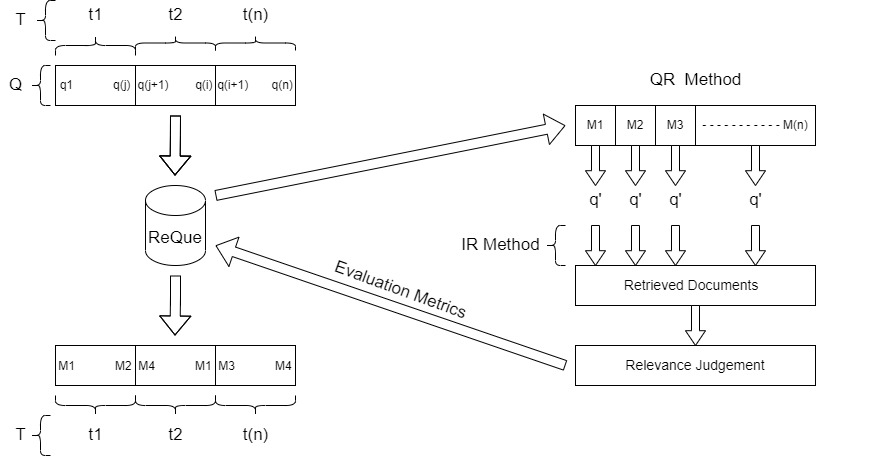
\includegraphics[width=0.8\columnwidth]{Images/image.png}
\caption{The diagram of our proposed method.\label{neural_net}}
\end{figure}

\subsection{Preprocess The Data Set}\label{topic_detection}
We use the TREC 2009 Million Query data set \cite{carterette2009million} as the input of our method. This data set consists of 40,000 queries with their relevance judgments. Only the query type of the 420 of the queries are identified. In this step, we delete unnecessary columns from the original data set and only keep query and query id as inputs. Table 1 shows the example of our input $\mathcal{Q}={q_1, q_2,..,q_n}$. We used the preprocessed form of the original data set to make it appropriate as an input for our next step, which we explain in the following section.

\begin{table}[h]
\begin{tabularx}{0.35\textwidth} { 
  | >{\raggedright\arraybackslash}X 
  | >{\centering\arraybackslash}X 
  | >{\centering\arraybackslash}X
  | >{\raggedright\arraybackslash}X | }
 \hline
20051 & cuttle fish bone \\
 \hline
20054  & 50plus \\
 \hline
20055  & usairway \\
\hline 
20065  & rock and gem shows \\
\hline 
\end{tabularx}
\caption{\label{tab:table-name}The input queries and their id }
\end{table}

\subsection{Evaluation Results of QR Methods}
We use the ReQue \cite{tamannaee2020reque} as a toolkit to pass our queries as an input and return the results of the evaluation of QR methods. ReQue consists of 3 main steps. First, use different query expander techniques as query refinements methods to generate new query ${q^'}$, given the ${q}\in\mathcal{Q}$. Table 2 illustrates the new queries for the initial queries based on QR methods. we also show the procedure of the ReQue in Figure 1.

\begin{table}[h]
\begin{tabularx}{0.43\textwidth} { 
  | >{\raggedright\arraybackslash}X 
  | >{\centering\arraybackslash}X 
  | >{\centering\arraybackslash}X
  | >{\raggedright\arraybackslash}X | }
 \hline
QR Method & Initial Query & New Query \\
 \hline
conceptnet  & rock and gem shows & music stone gem things \\
 \hline
conceptnet  & cuttle fish bone & cuttlefish animal A bass skeleton body part\\
\hline 
conceptnet  & 50plus & plus\\
\hline 
stem.krovetz  & rock and gem shows & rock and gem show \\
\hline
stem.krovetz  & cuttle fish bone & cuttle fish bone\\
\hline
stem.krovetz  & 50plus & plus\\
\hline
\end{tabularx}
\caption{\label{tab:table-name}The new queries are generated from initial query by using the different QR Method }
\end{table}

As Table 2 shows, some QR methods remove words from the original query or add new words to the original one, and some of them remain unchanged. Then, the new queries are used to retrieve documents using IR methods (e.g., bm25). Finally, evaluation metrics (e.g., MAP) are used to identify the relatedness of retrieved documents based on the given new query.


\subsection{Specify Suitable QR Method For Given Query Types}
So far, we have the evaluation results of QR methods for each input query. For our final step, we divided queries into different query types. Therefore, in each specific query type, we have queries with their QR methods evaluation. We ranked queries' evaluation results in each query type. The K-top query method will be selected as a nominated QR method for a given query type. 

In this research, we consider queries which are divided into the following categories: informational-open, which indicates the unspecific research need; informational-close refers to the specific research needs; the intention of navigational queries are finding a specific URL and resource which also called transactional queries are trying to find web-based resources like download the music\cite{carterette2009million}. $Algorithm 1$ shows the Pseudo-code for our proposed method.

\begin{algorithm}[h]
\caption{Finding suitable QR method for each query type}
\label{bicluster}
\begin{algorithmic}[1]
\Statex\textbf{Inputs:} 
\Statex\hspace{\algorithmicindent} set of $\mathbb{Q}={q_1, q_2... q_n}$, and its relevance judgement \Statex\textbf{Initialization:}
\Statex\hspace{\algorithmicindent} dividing queries $\mathbb{Q}={q_1, q_2... q_n}$ into different query types $\mathbb{T}={t_1, t_2... t_n}$
\Statex\hspace{\algorithmicindent} QR methods $\mathbb{M}={m_1, m_2... m_n}$ 
\Statex\textbf{Output:} ${m_n}\in\mathcal{M}$ for each ${t_n}\in\mathcal{T}$ 
\Procedure{find suitable $m_n$ for each $t_n$}{}
\ForAll{${q_n\in\mathcal{Q}}$}
\ForAll{${m_n\in\mathcal{M}}$}
\State ${q^'}\leftarrow{m(q)}$
\EndFor
\EndFor
\ForAll{${q^'}\in{Q^'}$}
\State {retrieved documents $d\leftarrow{IR Method({q^'})}$}
\EndFor
\Statex\hspace{\algorithmicindent} evaluation- results$\leftarrow{evaluation-metric(for all {q^'} and {d})}$
\Statex\hspace{\algorithmicindent}ranked $m\in\mathcal{M}$ for each $t\in\mathcal{M}$
\EndProcedure
\end{algorithmic}
\end{algorithm}


\bibliographystyle{ACM-Reference-Format}
\bibliography{bibliography.bib} 

\end{document}

